\documentclass[sigconf,nonacm]{acmart}

% meta-data -- adjust to meaningful values
\title{Project Report -- Group 10}
\author{???}
\author{???}


% remove overhead that is used in regular ACM papers
\settopmatter{printacmref=false} % box after abstract
\renewcommand\footnotetextcopyrightpermission[1]{} % copyright on first page
\pagestyle{plain} % running headers

\usepackage[utf8]{inputenc}
\usepackage[T1]{fontenc}
\usepackage{tikz}
\usetikzlibrary{shapes.geometric, arrows}

\tikzstyle{startstop} = [rectangle, rounded corners, minimum width=3cm, minimum height=1cm,text centered, draw=black, fill=red!30]
\tikzstyle{process} = [rectangle, minimum width=3cm, minimum height=1cm, text centered, draw=black, fill=orange!30]
\tikzstyle{decision} = [diamond, minimum width=3cm, minimum height=1cm, text centered, draw=black, fill=green!30]
\tikzstyle{arrow} = [thick,->,>=stealth]


\begin{document}

% The given structure is an example. Make sure that you adopt was have been
% requested in the assignment.

% \begin{abstract}
% % !TEX root =  ../report.tex
A clear and well-documented \LaTeX\ document is presented as an
article formatted for publication by ACM in a conference proceedings
or journal publication. Based on the ``acmart'' document class, this
article presents and explains many of the common variations, as well
as many of the formatting elements an author may use in the
preparation of the documentation of their work.

% \end{abstract}

\maketitle

% !TEX root =  ../report.tex
\section{Release Pipeline Documentation}
\section*{Release Pipeline Documentation for \texttt{lib-ml} Python Package}

This documentation provides a detailed description of the release pipeline used for publishing the \texttt{lib-ml} Python package to PyPI. The goal is to help new team members understand the pipeline steps, the tools used, and the flow of data and artifacts throughout the process. For a illustrative overview, see \autoref{fig:lib-ml-pipeline}.

\subsection{Pipeline Overview}

The release pipeline is triggered when a pull request (PR) is closed. It consists of two main jobs:

\begin{enumerate}
    \item \textbf{Test}: Runs tests on multiple environments to ensure the code is stable and functional.
    \item \textbf{Bump Version and Publish}: Bumps the package version, updates files, and publishes the package to PyPI.
\end{enumerate}

\subsection{Pipeline Steps}

\subsubsection{Testing (\texttt{test} job)}

\paragraph{Purpose}
Ensure the package works correctly in different environments and Python versions.

\paragraph{Implementation}
\begin{itemize}
    \item \textbf{Triggered}: When a pull request is merged.
    \item \textbf{Runs on}: Multiple OS and Python versions specified in a matrix.
    \item \textbf{Timeout}: 10 minutes.
\end{itemize}

\paragraph{Steps}
\begin{enumerate}
    \item \textbf{Checkout code}
    \begin{itemize}
        \item Uses \texttt{actions/checkout@v4}.
        \item Fetches the code from the merged pull request.
    \end{itemize}
    \item \textbf{Set up Python}
    \begin{itemize}
        \item Uses \texttt{actions/setup-python@v5}.
        \item Sets up the specified Python version from the matrix.
    \end{itemize}
    \item \textbf{Install Poetry}
    \begin{itemize}
        \item Installs Poetry using \texttt{pipx install poetry} or \texttt{pip install poetry}.
    \end{itemize}
    \item \textbf{Install dependencies}
    \begin{itemize}
        \item Runs \texttt{poetry install --with dev} to install development dependencies.
    \end{itemize}
    \item \textbf{Run tests}
    \begin{itemize}
        \item Executes \texttt{poetry run pytest} to run the test suite.
    \end{itemize}
\end{enumerate}

% \paragraph{Dataflow}
% \begin{itemize}
%     \item The merged code is checked out and set up with the specified Python environment.
%     \item Dependencies are installed, and tests are executed.
%     \item No artifacts are generated in this step but the outcome (pass/fail) determines if the next job will run.
% \end{itemize}

\subsubsection{Bump Version and Publish (\texttt{bump\_version\_and\_publish} job)}

\paragraph{Purpose}
Bump the package version, update the version in relevant files, and publish the package to PyPI.

\paragraph{Implementation}
\begin{itemize}
    \item \textbf{Triggered}: After the successful completion of the \texttt{test} job.
    \item \textbf{Runs on}: \texttt{ubuntu-latest}.
\end{itemize}

\paragraph{Steps}
Steps (1) to (4) are repeated before moving on to the next steps, which are:
\begin{enumerate}
    % \item \textbf{Checkout code}
    % \begin{itemize}
    %     \item Uses \texttt{actions/checkout@v4}.
    %     \item Fetches the code from the merged pull request.
    % \end{itemize}
    % \item \textbf{Set up Python}
    % \begin{itemize}
    %     \item Uses \texttt{actions/setup-python@v5}.
    %     \item Sets up Python 3.11.
    % \end{itemize}
    % \item \textbf{Install Poetry}
    % \begin{itemize}
    %     \item Installs Poetry using \texttt{pipx install poetry} or \texttt{pip install poetry}.
    % \end{itemize}
    % \item \textbf{Install dependencies}
    % \begin{itemize}
    %     \item Runs \texttt{poetry install --with dev} to install development dependencies.
    % \end{itemize}
    \item \textbf{Bump version and push tag}
    \begin{itemize}
        \item Uses \href{https://github.com/marketplace/actions/github-tag-bump}{\texttt{anothrNick/github-tag-action@1.67.0}}.
        \item Bumps the version and pushes a new tag to the repository.
        \item Environment variables used:
        \begin{itemize}
            \item \texttt{GITHUB\_TOKEN}: Token for accessing GitHub.
            \item \texttt{DEFAULT\_BUMP}: Default version bump type (\texttt{patch}).
            \item \texttt{TAG\_CONTEXT}: Context for tagging (\texttt{branch}).
            \item \texttt{WITH\_V}: Whether to include 'v' in the version tag (false).
            \item \texttt{PRERELEASE}: Pre-release flag (false).
        \end{itemize}
    \end{itemize}
    \item \textbf{Update files with new version}
    \begin{itemize}
        \item Runs \texttt{poetry run bump-my-version replace --config-file pyproject.toml --new-version \$(git describe --tags --abbrev=0)}.
        \item Updates the version in the \texttt{pyproject.toml} file.
    \end{itemize}
    \item \textbf{Build and publish to PyPI}
    \begin{itemize}
        \item Runs \texttt{poetry publish --build -u \_\_token\_\_ -p \${{ secrets.PYPI\_API\_KEY }}} to build and publish the package to PyPI.
        \item Uses \texttt{PYPI\_API\_KEY} secret for authentication.
    \end{itemize}
\end{enumerate}

% \paragraph{Dataflow}
% \begin{itemize}
%     \item The merged code is checked out again.
%     \item The Python environment is set up, and dependencies are installed.
%     \item The version is bumped, and the new tag is pushed to the repository.
%     \item The \texttt{pyproject.toml} file is updated with the new version.
%     \item The package is built and published to PyPI.
% \end{itemize}

\subsection{Artifacts and Data Flow}

\begin{enumerate}
    \item \textbf{Source Code}: Checked out from the merged pull request.
    \item \textbf{Python Environment}: Set up using specified versions from the matrix.
    \item \textbf{Dependencies}: Installed using Poetry.
    \item \textbf{Test Results}: Determines if the publish job should proceed.
    \item \textbf{Version Tag}: Created and pushed to the repository.
    \item \textbf{Updated \texttt{pyproject.toml}}: Contains the new version.
    \item \textbf{Published Package}: The final artifact, published to PyPI.
\end{enumerate}

\subsection{Tools Used}

\begin{itemize}
    \item \textbf{GitHub Actions}: CI/CD platform for running workflows.
    \item \textbf{Poetry}: Dependency management and packaging tool.
    \item \textbf{pytest}: Testing framework.
    \item \href{https://github.com/marketplace/actions/github-tag-bump}{\textbf{anothrNick/github-tag-action}: Action for tagging releases.}
\end{itemize}

\begin{figure}[h!]
    \centering
    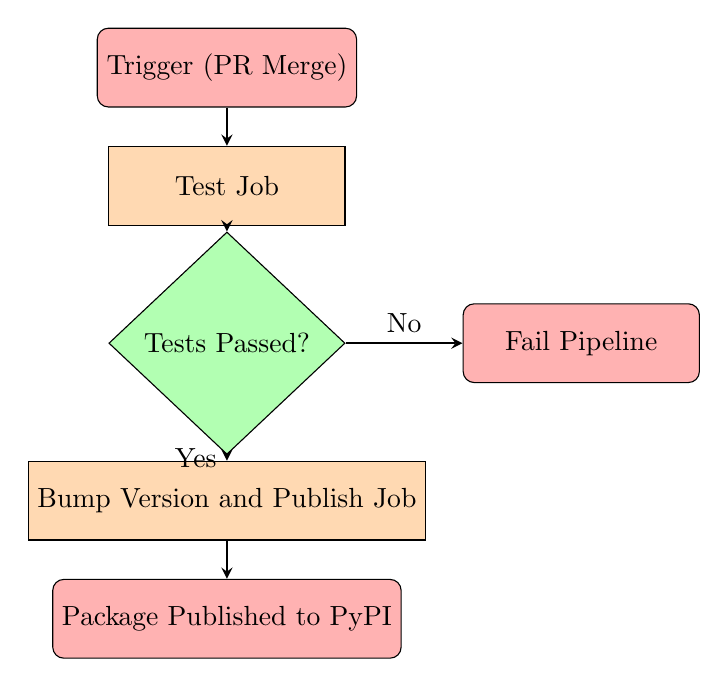
\begin{tikzpicture}[node distance=1.5cm]
        \node (start) [startstop] {Trigger (PR Merge)};
        \node (test) [process, below of=start] {Test Job};
        \node (decision1) [decision, below of=test, yshift=-0.5cm] {Tests Passed?};
        \node (bumpversion) [process, below of=decision1, yshift=-0.5cm] {Bump Version and Publish Job};
        \node (stop) [startstop, below of=bumpversion] {Package Published to PyPI};
        \node (fail) [startstop, right of=decision1, xshift=3cm] {Fail Pipeline};

        \draw [arrow] (start) -- (test);
        \draw [arrow] (test) -- (decision1);
        \draw [arrow] (decision1) -- node[anchor=east] {Yes} (bumpversion);
        \draw [arrow] (bumpversion) -- (stop);
        \draw [arrow] (decision1) -- node[anchor=south] {No} (fail);
    \end{tikzpicture}
    \label{fig:lib-ml-pipeline}
    \caption{Flowchart of \texttt{lib-ml} Python Package Release Pipeline}
\end{figure}

% \begin{figure}[h!]
%     \centering
%     \begin{tikzpicture}[node distance=1.5cm]
%         \node (source) [process] {Source Code};
%         \node (env) [process, below of=source] {Python Environment};
%         \node (deps) [process, below of=env] {Dependencies};
%         \node (tests) [process, below of=deps] {Test Results};
%         \node (version) [process, below of=tests] {Version Tag};
%         \node (pyproject) [process, below of=version] {Updated \texttt{pyproject.toml}};
%         \node (package) [process, below of=pyproject] {Published Package};
        
%         \draw [arrow] (source) -- (env);
%         \draw [arrow] (env) -- (deps);
%         \draw [arrow] (deps) -- (tests);
%         \draw [arrow] (tests) -- (version);
%         \draw [arrow] (version) -- (pyproject);
%         \draw [arrow] (pyproject) -- (package);
%     \end{tikzpicture}
%     \caption{Data Flow Diagram of \texttt{lib-ml} Python Package Release Pipeline}
% \end{figure}

\section*{Release Pipeline Documentation for \texttt{model-service} Container Image}

This documentation provides a detailed description of the release pipeline used for publishing the \texttt{model-service} container image. Also here, the goal is to help new team members understand the pipeline steps, the tools used, and the flow of data and artifacts throughout the process. For a illustrative overview, see \autoref{fig:model-service-pipeline}.

\subsection{Pipeline Overview}

The release pipeline is triggered when a new tag matching the pattern \texttt{v[0-9]+.[0-9]+.[0-9]+} is pushed to the repository. It consists of a single job:

\begin{enumerate}
    \item \textbf{Build}: Builds the Docker image and pushes it to the GitHub Container Registry (GHCR).
\end{enumerate}

\subsection{Pipeline Steps}

\subsubsection{Build (\texttt{build} job)}

\paragraph{Purpose}
Build the Docker image for the \texttt{model-service} and push it to the GitHub Container Registry (GHCR).

\paragraph{Implementation}
\begin{itemize}
    \item \textbf{Triggered}: When a tag matching the pattern \texttt{v[0-9]+.[0-9]+.[0-9]+} is pushed.
    \item \textbf{Runs on}: \texttt{ubuntu-22.04}.
\end{itemize}

\paragraph{Steps}
\begin{enumerate}
    \item \textbf{Checkout code}
    \begin{itemize}
        \item Uses \texttt{actions/checkout@v4}.
        \item Checks out the code from the repository.
    \end{itemize}
    \item \textbf{Parse version info from tag}
    \begin{itemize}
        \item Runs a shell script to parse the version information from the tag.
        \item Extracts the major, minor, and patch version numbers.
        \item Sets the parsed version numbers as environment variables.
    \end{itemize}
    \item \textbf{Registry Login (ghcr.io)}
    \begin{itemize}
        \item Logs into the GitHub Container Registry (GHCR) using the \texttt{GH\_TOKEN} secret.
        \item Uses the GitHub Actions context for authentication.
    \end{itemize}
    \item \textbf{Build and Push Docker Image}
    \begin{itemize}
        \item Builds the Docker image using the Dockerfile in the repository.
        \item Tags the image with:
        \begin{itemize}
            \item Full version (e.g., \texttt{v1.2.3}).
            \item Major and minor version with \texttt{.latest} suffix (e.g., \texttt{1.2.latest}).
            \item Major version with \texttt{.latest} suffix (e.g., \texttt{1.latest}).
            \item \texttt{latest} tag.
        \end{itemize}
        \item Pushes all tagged images to the GitHub Container Registry.
    \end{itemize}
\end{enumerate}

% \paragraph{Dataflow}
% \begin{itemize}
%     \item The source code is checked out from the repository.
%     \item The version information is parsed from the tag and set as environment variables.
%     \item The Docker image is built and tagged with multiple tags.
%     \item The Docker image is pushed to the GitHub Container Registry with all the tags.
% \end{itemize}

\subsection{Artifacts and Data Flow}

\begin{enumerate}
    \item \textbf{Source Code}: Checked out from the repository.
    \item \textbf{Docker Image}: Built from the source code.
    \item \textbf{Version Tags}: Parsed from the pushed tag and used to tag the Docker image.
    \item \textbf{Published Image}: The final artifact, pushed to the GitHub Container Registry.
\end{enumerate}

\subsection{Tools Used}

\begin{itemize}
    \item \textbf{GitHub Actions}: CI/CD platform for running workflows.
    \item \textbf{Docker}: Containerization platform for building and pushing images.
    \item \textbf{GitHub Container Registry (GHCR)}: Registry for storing and managing Docker container images.
\end{itemize}

\begin{figure}[h!]
    \centering
    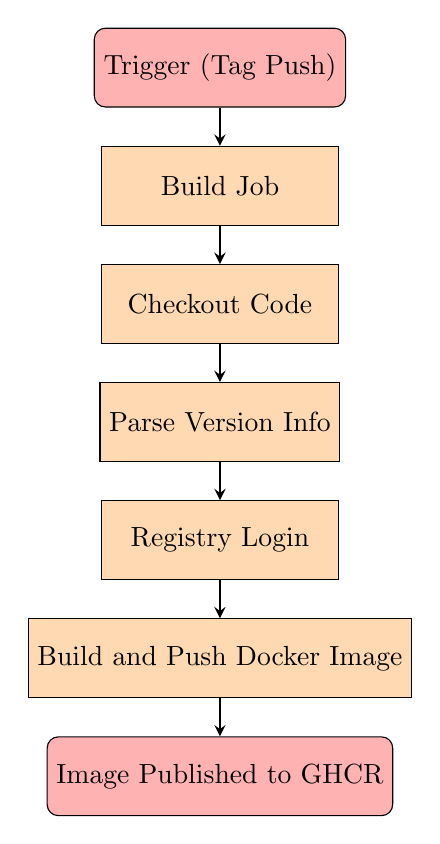
\begin{tikzpicture}[node distance=1.5cm]
        \node (start) [startstop] {Trigger (Tag Push)};
        \node (build) [process, below of=start] {Build Job};
        \node (checkout) [process, below of=build] {Checkout Code};
        \node (parse) [process, below of=checkout] {Parse Version Info};
        \node (login) [process, below of=parse] {Registry Login};
        \node (docker) [process, below of=login] {Build and Push Docker Image};
        \node (stop) [startstop, below of=docker] {Image Published to GHCR};
        
        \draw [arrow] (start) -- (build);
        \draw [arrow] (build) -- (checkout);
        \draw [arrow] (checkout) -- (parse);
        \draw [arrow] (parse) -- (login);
        \draw [arrow] (login) -- (docker);
        \draw [arrow] (docker) -- (stop);
    \end{tikzpicture}
    \caption{Flowchart of \texttt{model-service} Container Image Release Pipeline}
    \label{fig:model-service-pipeline}
\end{figure}
% !TEX root =  ../report.tex
\begin{figure*}[ht!]
    \centering
    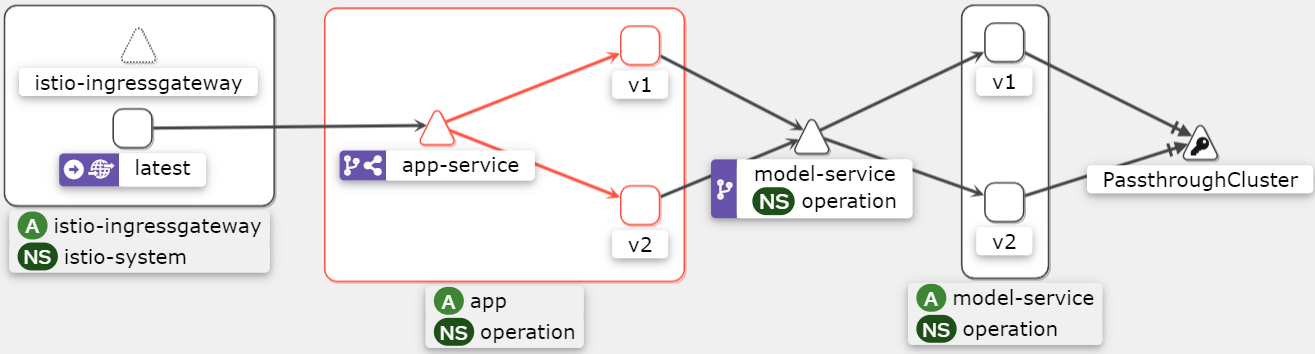
\includegraphics[width=18cm]{report/images/kiali.png}
    \caption{Deployment of operation}
    \label{fig:kiali}
\end{figure*}
\begin{figure*}[!ht]
    \centering
    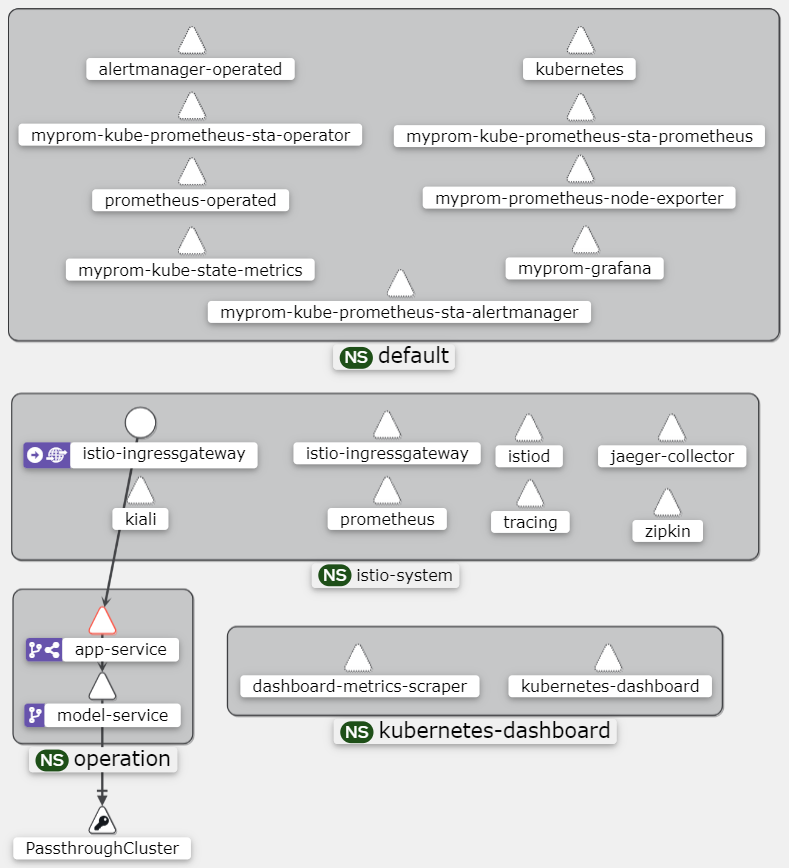
\includegraphics[width=13cm]{report/images/kialiServices.png}
    \caption{Entire deployment cluster}
    \label{fig:kialiall}
\end{figure*}
\clearpage
\section{Deployment Documentation}
This section covers the deployment and data flow of the project. The project is deployed on a minikube cluster, this allows for scaling of the project as well as stability through backup deployment replicas.

\subsection{Deployment structure}
The deployment structure is visualized in \autoref{fig:kiali}. It consists of two main services with each having two deployment versions for a potential canary release:

\begin{enumerate}
    \item \textbf{app-service}: App-service handles the front-end of the application and serves the page that the user directly interacts with. This is done through two flask deployments each running a different version. Each of these deployments consist of only 1 replica and therefore do not provide redundancy out of the box. This can be scaled up to improve availability.
    \item \textbf{model-service}: Model-service handles the back-end of the application and provides the "predict" endpoint for the app to interact with, which returns the prediction result given an url. This is done through two flask deployments hosting the model each running a different version. Each of these deployments also consist of only 1 replica.
\end{enumerate}


\subsection{Data flow}
The Ingress gateway is provided by Istio and serves as the entry point to the application. The request is then handled by the app-service which forwards the request to one of the two deployment versions with equal probability (50/50). The user is then able to make a prediction on the app. The app then sends a post request to the model-service which forwards it to the corresponding model-service deployment version. The prediction is then directly returned through the passthrough cluster.

\subsection{Full cluster deployment}
The project furthermore employs various monitoring tools on the cluster, these include Prometheus and Grafana. Additionally various other dashboards can be added to the cluster such as the Minikube, Jaeger and Kiali dashboard. The full deployment of all clusters can be found in \autoref{fig:kialiall}. Prometheus scrapes the "/metrics" endpoint of the model-service deployments to keep track of various metrics. Grafana can then be connected to prometheus to provide a intuitive dashboard of the various metrics.



% !TEX root =  ../report.tex
\section{Extension Proposal}
During the project, we experienced issues with setting up the software environment using Ansible and Vagrant. These issues became apparent as we had to do a more complex task by connecting the virtual machines and setting up the Kubernetes cluster for the virtual machines. The goal of Ansible is to provision a local software environment together with Vagrant, which enables the software to run locally on virtual machines. This should remove the \textit{it runs on my machine} argument by providing a stable and reproducible environment. As a result, software development should speed up. However, during the development process, we noticed that using Ansible instead slowed down development due to several issues we encountered. Following our discussion of the issues, we will explore two development approaches that could be used to address them.

\paragraph{Issues}
In this paragraph, we will discuss some issues that we experienced personally. During development, Ansible sometimes breaks despite no apparent changes in the local environment. Different inventory.cfg files might be required depending on the developer's operating system, which hurts reproducibility. Command outputs have limited verbosity or the verbosity can be needlessly complex, and playbook execution can have very long wait times\cite{ansible-slow}. Additionally, some commands that run successfully when executed directly via SSH do not work in the playbook. Configuration setup options are also limited and sometimes difficult to implement, due to Ansible using a different thread for every command. As discussed in this blog by Eric Hu, Ansible seems better for setting up applications than for configuration management (e.g. setting up a Kubernetes cluster)\cite{ansible-comparison}. This was something we experienced ourselves as well, as Ansible creates a new shell when executing a command. As a result, the inexperienced user can lose environment and/or configuration settings when executing commands sequentially\cite{ansible-shell}. Even though it is certainly possible to configure a complex environment with Ansible, it might not be the best tool for our specific job.

\subsection{Deployment of an In-House Cluster}
One of the use cases for this setup could be to run an in-house application on a local company network. Vagrant and Chef can be used to provision this server to allow for easy scaling. Docker-compose will be used for local development. Especially the continuous deployment features of Chef can be useful in this case\cite{ansible-vs-chef2}. Even though Ansible has some strong features, especially the good security using SSH and its ease of use Chef is likely a better option here. Because Chef is a more mature technology\cite{ansible-vs-chef}, has better configuration management and better deployment features. Furthermore, because Chef works well with our current CI/CD pipelines, if a new version of the software is created it can immediately be used in the company network. 

\begin{figure}
    \centering
    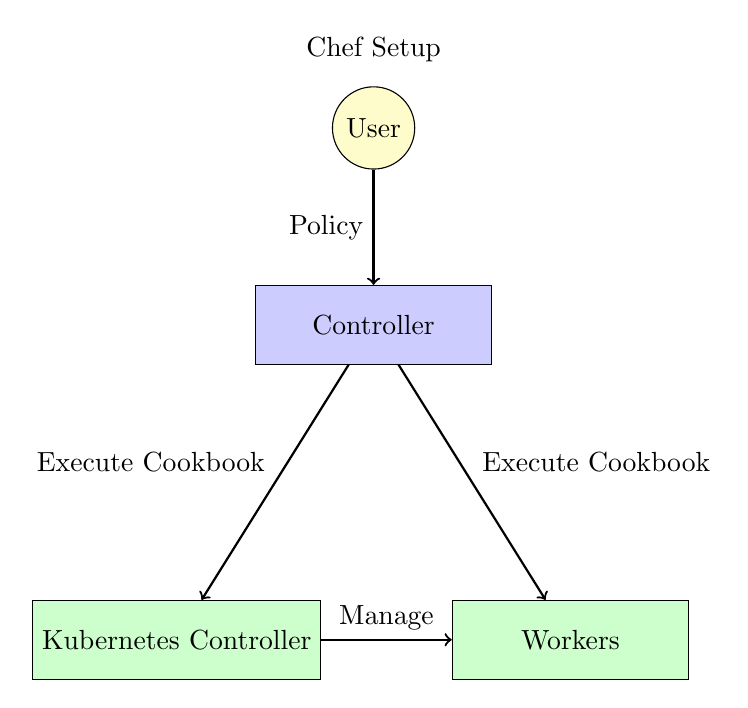
\begin{tikzpicture}
    
    % Draw the user
    \node[draw, circle, minimum size=1cm, fill=yellow!20] (user) at (0, 2.5) {User};
    
    % Draw the controller
    \node[draw, rectangle, minimum width=3cm, minimum height=1cm, fill=blue!20] (controller) at (0, 0) {Controller};
    
    % Draw the workers
    \node[draw, rectangle, minimum width=3cm, minimum height=1cm, fill=green!20] (worker1) at (-2.5, -4) {Kubernetes Controller};
    \node[draw, rectangle, minimum width=3cm, minimum height=1cm, fill=green!20] (workerN) at (2.5, -4) {Workers};
    
    % Draw connections
    \draw[->, thick] (user) -- node[midway, left] {Policy} (controller);
    \draw[->, thick] (controller) -- node[midway, above left] {Execute Cookbook} (worker1);
    \draw[->, thick] (controller) -- node[midway, above right] {Execute Cookbook} (workerN);
    \draw[->, thick] (worker1) --node[midway, above] {Manage} (workerN);
    % Optional: Add labels
    \node at (0, 3.5) {Chef Setup};
    % \node at (0, -5.5) {Executing Cookbooks};
    
    \end{tikzpicture}
    \caption{Example Chef Infrastructure}
    \label{fig:chef-infrastructure}
\end{figure}

% \subsection{Moving to a Bigger Scale}
% If the goal of the development would be 
% Local Development within an Ansible-Provisioned Machine and Migrating to the Cloud.





% Some of these were: different inventory.cfg needed for different local operating systems, some commands that could be executed locally displaying different behavior in the playbook, it being hard to update machine system configurations, limited verbosity in command outputs and very long wait times\cite{ansible-slow}. 

% At the end of the assignments, there is a complete local development environment. In this environment we can provision machines

% At the end of this project, we have a fairly complete local development environment. If this were a real-life situation, one would want to migrate the functionality we have created to an environment which a lot of people can use. 



\bibliographystyle{ACM-Reference-Format}
\bibliography{references}

\end{document}
\endinput
